\subsection{Load}
\label{sec:Loadsystem_load}
The Load serves no other function than converting generated electrical energy to thermic energy (heat). This is done by using power resistors. But then this is saying it impotent to choose the right setup.

\large List of things that has to be in order before using the load system!
\begin{itemize}
	\item {Generator}
	\subitem \textit{Must not exceed the power limit.}
	\subitem \textit{Must not exceed the speed limit.}
	\subitem \textit{the power limit must be greater or match the Test objects Power usage.}
	\item {Load resistor}
	\subitem \textit{Must not exceed the power limit with a voltage equal the nominal voltage.}
\end{itemize}

To get all these thing in order, some math has to been made. \\
First step is to find all information about the load systems components: 

\lstset{language=MATLAB}
\begin{lstlisting}
%% Constants

R_a             = 0.103;           % Anchor resistance (Ohm)
R_load          = 2.2;             % Load resistor (Ohm)
Kt              = 38.5*10^(-3);    % Torque Constant (Nm/A)
Gear            = 4.3;             % Gearing ratio in the motor (gg)
RR_r            = 0.076;           % RollingRoad radius (m)
Kb_rpm          = 248;             % Speed constant (rpm/V)
Kb              = Kt;              % Speed constant (rad/V)
AU2_peak_speed  = 30;              % AU2 peak speed (km/h)
V_N             = 24;              % Nominal Voltage (V)

%% limits

Generator_max_speed     = 9500;     %(rpm)
MAX_Continuous_current  = 10.8;     %(A)
Max_watt                = 200;      %(W)
R_load_max_watt         = 250;      %(W)
\end{lstlisting}

Note: There has been made a script that automatic calculate the best setup. (LoadSystem.m)\fxnote{mangler reference}.

The next step is to see how fast the Rolling Road is gonna rotate, then a test object are on it. In this example the test object is AU2. Then done the question is. Are there a need for gear-set to get a better rotating speed to generate a voltage what is closer to the nominal voltage?

\lstset{language=MATLAB}
\begin{lstlisting}
%% Calculation
% First is to find out what speed the generator is running.

% Rollings road max rotating speed (rpm)
RR_max_speed = AU2_peak_speed * KmToRpm 

% Voltage generated by the generator
% without gear
RR_Vb_nogear_max    = RR_max_speed * Kb_rpm^-1
% with gear
RR_Vb_gear_max      = RR_max_speed * Gear * Kb_rpm^-1
\end{lstlisting}

The result from this part is:

\begin{equation}
\begin{split}
	RR_{max_{speed}} = \SI{1047}{rpm}\\
	RR_{Vb_{nogear_max}} = \SI{4.22}{\volt}\\
	RR_{Vb_{gear_max}} = \SI{18.15}{\volt}
\end{split}
\end{equation}

It is clear. Gear option is the best option because it is closer to the nominal voltage.

The next step is to find out the best setup of the power resistor. With some calculation the best result is using two power resistor parallel. 

\lstset{language=MATLAB}
\begin{lstlisting}
% find the optimal resistor load setup.

Load_setup = [(R_load^2)/(R_load*2)+R_a, Max_watt*2; R_load+R_a, Max_watt; R_load*2+R_a, Max_watt*2];

best = 1;
for i = [1:length(Load_setup)]
if (RR_Vb_max^2 / Load_setup(i,1) <= Max_watt) && (Load_setup(i,2) > RR_Vb_max^2 / Load_setup(best,1)) && (RR_Vb_max^2 / Load_setup(i,1) > RR_Vb_max^2 / Load_setup(best,1))
best = i; 
end
end

Load_setup(best,1)
Power_max = RR_Vb_max^2 / Load_setup(best,1)
I_max = RR_Vb_max / Load_setup(best,1)
\end{lstlisting}


\begin{equation}
	\begin{split}
		R_{load} &= \SI{1.203}{\Omega}\\
		Power_{max} &= \SI{273.98}{\watt}\\
		I_{max} &= \SI{15.09}{A}
	\end{split}
\end{equation}

Have to notify that this is not possible because it will cause a melt down of the Rolling Road. That will result in max use of $ 73 \% $ then it runs at top speed!\\

After the limitation and calculate with $ Power_{max} = \SI{200}{\watt} $. The max torque, force and current can be calculated.

\lstset{language=MATLAB}
\begin{lstlisting}
% max torque, force and current.

I_max = (Power_max/RR_Vb_max)

torque_generator = (Power_max/RR_Vb_max) * Kt

if gear
torque_max = (Power_max/RR_Vb_max) * Kt * Gear
force_max = torque_max / RR_r
else
torque_max = (Power_max/RR_Vb_max) * Kt
force_max = torque_max / RR_r
end
\end{lstlisting}

The last results:
\begin{equation}
\begin{split}
Power_{max} &= \SI{200}{\watt}\\
I_{max} &= \SI{11.02}{A}\\
torque_{generator} &= \SI{0.42}{\newton \metre}\\
torque_{max} &= \SI{1.82}{\newton \metre}\\
force_{max} &= \SI{24.00}{\newton}
\end{split}
\end{equation}

\begin{figure}[H]
	\centering
	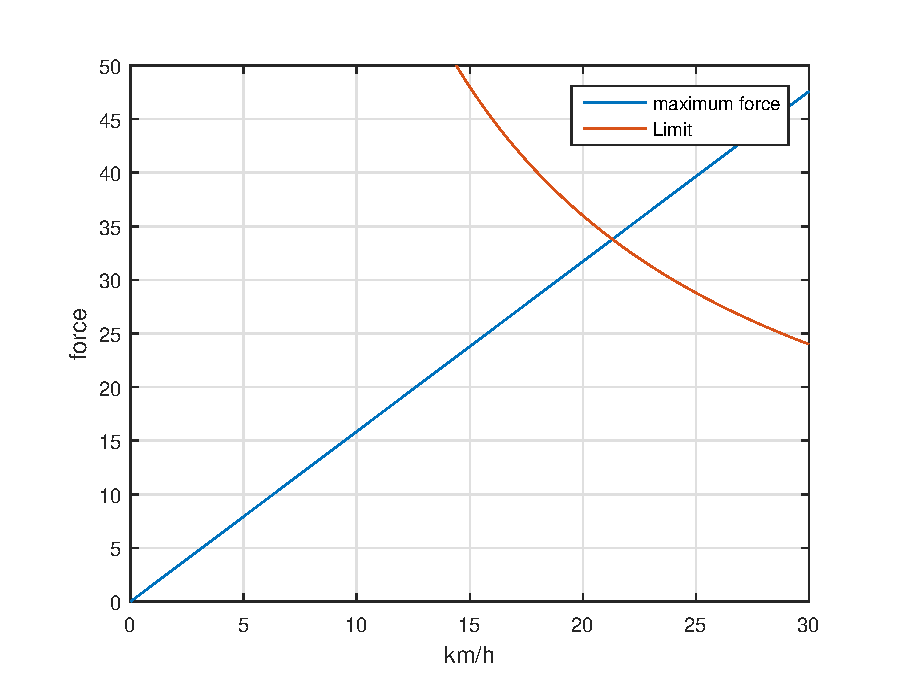
\includegraphics [width=4in]{Hardware/Pictures/force.eps}
	\caption{This diagram give shows how much force that maximum can get from a speed with this setup. The other line shows where 200 W limit is.}
	\label{fig:Force_and_speed}
\end{figure}